% !Mode:: "TeX:UTF-8"
\documentclass[10pt,punct]{ctexbeamer}
%\usepackage[utf8]{inputenc}
% fontset=mac
\usefonttheme[onlymath]{serif}


\usepackage{amsmath,amssymb,amsthm}             % AMS Math
%\usepackage[T1]{fontenc}
\usepackage{graphicx}
\usepackage{epstopdf}
\usepackage{tikz}
\linespread{1.3}

\usepackage{mathrsfs}  %花写字母
\usepackage{colortbl}  %彩色表格需要加载的宏包

%%%=== theme ===%%%
% \usetheme{Warsaw}
%\usetheme{Copenhagen}
%\usetheme{Singapore}
\usetheme{Madrid}
%\usefonttheme{professionalfonts}
%\usefonttheme{serif}
% \usefonttheme{structureitalicserif}
%%\useinnertheme{rounded}
%%\useinnertheme{inmargin}
\useinnertheme{circles}
%\useoutertheme{miniframes}
\setbeamertemplate{navigation symbols}{}
\setbeamertemplate{footline}[frame number]

\titlegraphic{
\includegraphics[width=2cm]{../tjnu.jpg}}

%\usepackage[fontset=mac]{ctex}
%\usepackage{ctex}
% \usepackage{CJK,CJKnumb,CJKulem}
%\usepackage{minitoc}


\setbeamertemplate{theorems}[numbered]
\newtheorem{thm}{定理}
\newtheorem{lem}{引理}
\newtheorem{ex}{例}
\newtheorem*{theo}{定理}
\newtheorem*{conj}{猜想}
\newtheorem*{defi}{定义}
\newtheorem*{coro}{推论}
\newtheorem*{rem}{注}
\newtheorem*{prop}{性质}
\newtheorem{pr1}{性质}
\newtheorem{pr2}{性质}
\newtheorem{pr3}{性质}
\newtheorem*{qst}{问题}

\def\qed{\nopagebreak\hfill{\rule{4pt}{7pt}}\medbreak}
\def\pf{{\bf 证明~~ }}
\def\sol{{\bf 解~~ }}



\def\R{\mathbb{R}}
\def\Rn{\mathbb{R}^n}
\def\A{\mathscr{A}}
\def\B{\mathscr{B}}
\def\D{\mathscr{D}}
\def\E{\mathscr{E}}
\def\O{\mathscr{O}}
\def\e{\mathrm{e}}
\def\i{\, \mathrm{i}}

\def\rank{\operatorname{rank}}
\def\dim{\operatorname{dim}}
\def\0{\mathbf{0}}
\def\a{\alpha}
\def\b{\beta}
\def\r{\gamma}

\usepackage{graphicx}
\usepackage{color}
\definecolor{linkcol}{rgb}{0,0,0.4}
\definecolor{citecol}{rgb}{0.5,0,0}

\definecolor{blue}{rgb}{0,0.08,1}
\newcommand{\blue}{\textcolor{blue}}


%  \DeclareGraphicsExtensions{.eps}
%   \usepackage[a4paper,pagebackref,hyperindex=true,pdfnewwindow=true]{hyperref}


\begin{document}



\title[]{习近平总书记关于科技创新的重要论述}
\author[]{{\large 张彪} }
\institute[]{{\normalsize
		天津师范大学\\[4pt]
        数学科学学院\\[10pt]
		zhang@tjnu.edu.cn}}

\date{}



\AtBeginSection[]
{
\begin{frame}
	\frametitle{提纲}
	\tableofcontents[currentsection]
\end{frame}
}



\begin{frame}
\maketitle
\end{frame}

\begin{frame}
\frametitle{\textcolor{orange}{提纲}}
\tableofcontents
\end{frame}





\section{引言}


\begin{frame}{习近平总书记关于“科技创新”的重要讲话}
\begin{block}{2018年5月2日在北京大学考察时的讲话}
     重大科技创新成果是国之重器、国之利器, 必须牢牢掌握在自己手上, 必须依靠自力更生、自主创新.
\end{block}

\begin{block}{2020年10月16日在中央政治局第二十四次集体学习时的讲话}
 当今世界正经历百年未有之大变局, 科技创新是其中一个关键变量. 我们要于危机中育先机、于变局中开新局, 必须向科技创新要答案.
\end{block}
\end{frame}

\begin{frame}{二十大报告将教育、科技、人才统筹部署}

\begin{itemize}
\item \blue{坚持科技是第一生产力、人才是第一资源、创新是第一动力, }
\item \blue{深入实施科教兴国战略、人才强国战略、创新驱动发展战略, }
\item \blue{开辟发展新领域新赛道, 不断塑造发展新动能新优势. }
\end{itemize}

\end{frame}




%\begin{frame}
%
%\begin{columns}[c]  %开始进入分栏环境, 居中设置
%
%	\column{6cm}
%\begin{leftline}
%	{\Large  宇宙之大, 粒子之微, } \\[8pt]
%
%	{ \Large 火箭之速, 化工之巧, }\\[8pt]
%
%	{ \Large 地球之变, 生物之谜, }\\[8pt]
%
%	{ \Large 日用之繁, 无处不用数学. }
%\end{leftline}
%
%\rightline{ {\Large 一华罗庚 \qquad \qquad\qquad}}
%	\column{6cm}
%	\begin{figure}[p]
%		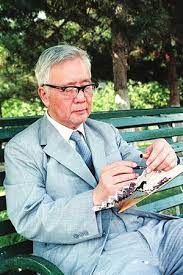
\includegraphics[scale=0.5]{hua.jpeg}
%		\caption{华罗庚 (1910--1985)}
%	\end{figure}
%中国解析数论创始人和开拓者
%\end{columns}
%\end{frame}



\begin{frame}

	\begin{columns}[c]  %开始进入分栏环境, 居中设置

		\column{6cm}
     \begin{itemize}
         \item 培养了包括廖山涛、吴文俊、丘成桐、郑绍远, 李伟光等在内的著名数学家.
         \item
         1981年至1984年任美国国家数学科学研究所(MSRI)首任所长.

         \item 1984年至1992年任天津南开数学研究所首任所长.
         \item 1992年~2004年, 陈省身任天津南开数学研究所名誉所长.

        \item  2004年12月, 陈省身在天津医科大学总医院逝世, 享年93岁.
     \end{itemize}


		\column{6.5cm}
		\begin{figure}[p]
			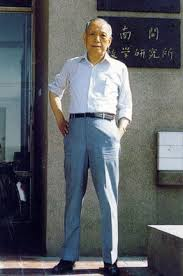
\includegraphics[scale=0.6]{chern.jpeg}
					\caption{陈省身 (1911-2004)}
%{\small	20世纪世界最重要的微分几何学家之一、\\
%美国国家数学科学研究所首任所长、\\
%南开数学研究所首任所长	}
    \end{figure}
	\end{columns}


\end{frame}


\begin{frame}

        \begin{figure}[p]
            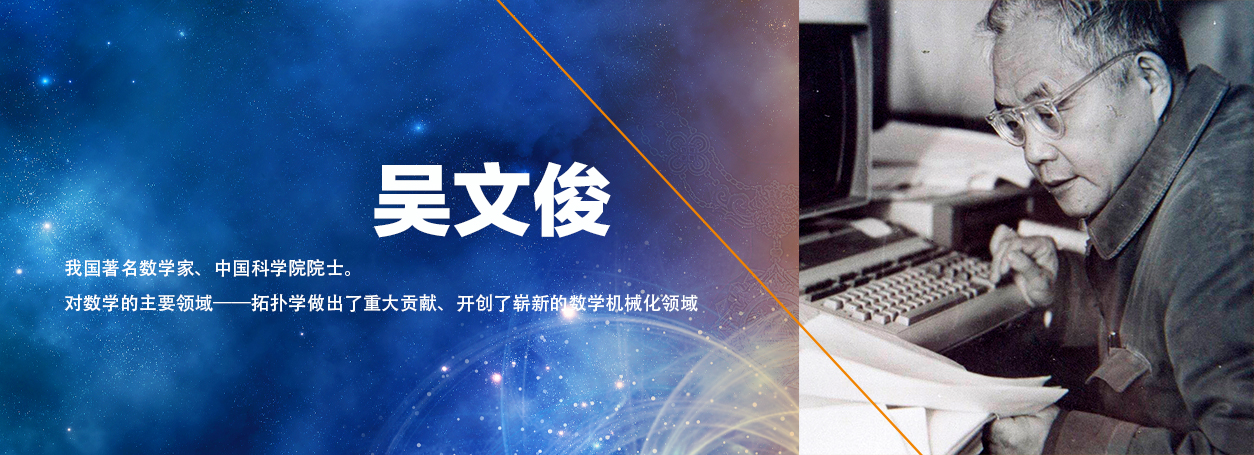
\includegraphics[scale=0.3]{wu.jpeg}
            \caption{吴文俊(1919-2017), 中国科学院数学与系统科学研究院研究员}
        \end{figure}
    \small{
\begin{itemize}
\item 吴文俊对数学的核心领域拓扑学做出了重大贡献他为拓扑学做了奠基性的工作;他的示性类和示嵌类研究被国际数学界称为“吴公式”, “吴示性类”, “吴示嵌类”, 至今仍被国际同行广泛引用.

\item 吴文俊 开创了数学机械化新领域, 对数学与计算机科学研究影响深远.


\item 2000年, 吴文俊获得首届最高国家科学技术奖.

\item 2019年, 吴文俊被授予了“人民科学家”的国家荣誉称号.

\end{itemize}}
\end{frame}


\section{行列式的几何解释}

\begin{frame}{平行四边形的面积}
已知 $\overrightarrow{O A}=\left(\begin{array}{l}a_1 \\ a_2\end{array}\right), \overrightarrow{O B}=\left(\begin{array}{l}b_1 \\ b_2\end{array}\right)$.


求$O A, O B$ 为一组邻边的平行四边形OAPB 的面积?

        \begin{figure}[p]
    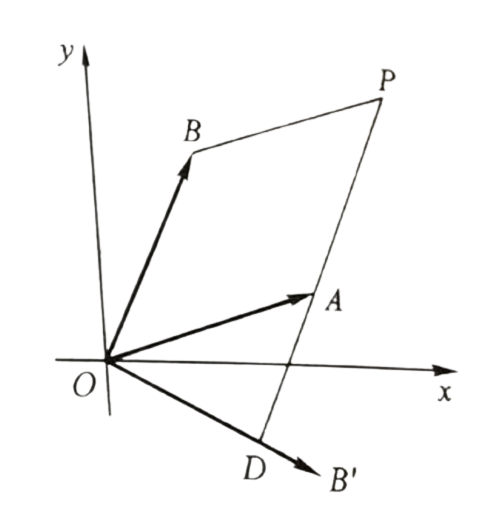
\includegraphics[scale=0.6]{det-2.png}
    %    \caption{}
\end{figure}

\end{frame}

\begin{frame}
    \begin{columns}[c]
        \column{8cm}

        对任意 $\overrightarrow{O A}=\left(\begin{array}{l}a_1 \\ a_2\end{array}\right), \overrightarrow{O B}=\left(\begin{array}{l}b_1 \\ b_2\end{array}\right)$

        将 $O B$ 绕 $O$ 沿顺时针方向旋转直角得到有向线 段 $O B^{\, \prime}$. 则 $\overrightarrow{O B^{\, \prime}}=\left(\begin{array}{r}b_2 \\ -b_1\end{array}\right)$.


        %则 $\overrightarrow{O B^{\, \prime}}=\left( b_2, -b_1 \right)$.

        考虑$\Delta=a_1 b_2-a_2 b_1$, 它就是 $\overrightarrow{O A} \cdot \overrightarrow{O B^{\, \prime}}$.

        由于 $\left|O B^{\, \prime}\right|=|O B|, \angle B O B^{\, \prime}=$ $-\frac{\pi}{2}$, 于是
%        \pause
        $$
        \begin{aligned}
            \Delta=\overrightarrow{O A} \cdot \overrightarrow{O B^{\, \prime}}
            & = |O A|\left|O B^{\, \prime}\right| \cos \angle A O B^{\, \prime}\\
            & = |O A||O B| \cos \left(\angle A O B-\frac{\pi}{2}\right) \\
            & = |O A||O B| \sin \angle A O B
        \end{aligned}
        $$


        \column{4.5cm}
        \begin{figure}[p]
            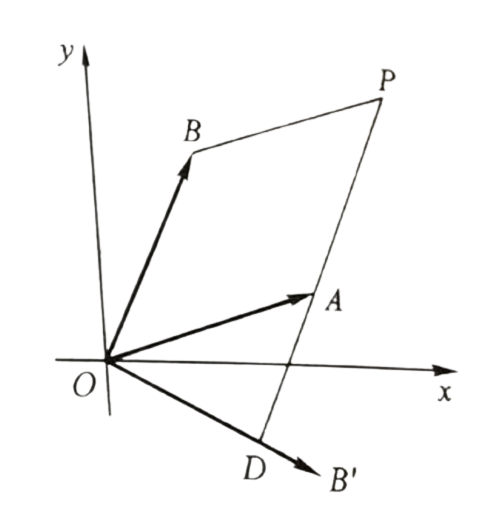
\includegraphics[scale=0.4]{det-2.png}
            %    \caption{}
        \end{figure}

        \pause
        \begin{itemize}
            \item  $\triangle$ 的\alert{绝对值}就是以 $O A, O B$ 为一组邻边的平行四边形OAPB 的面积
            \item   $\triangle$ 的\alert{符号}就是 $\sin \angle A O B$ 的符号
        \end{itemize}


    \end{columns}



\end{frame}

\begin{frame}{平行四边形的面积与二阶行列式}


    对任意 $\overrightarrow{O A}=\left(\begin{array}{l}a_1 \\ a_2\end{array}\right), \overrightarrow{O B}=\left(\begin{array}{l}b_1 \\ b_2\end{array}\right)$, 定义 $$\operatorname{det}(\overrightarrow{O A}, \overrightarrow{O B})=|O A||O B| \sin \angle A O B$$

    也记作
    $$\operatorname{det}\left(\begin{array}{ll}a_1 & b_1 \\ a_2 & b_2\end{array}\right) \mbox{ 或  } \quad \left|\begin{array}{ll}a_1 & b_1 \\ a_2 & b_2\end{array}\right|$$


    称为\alert{二阶行列式}.

    将它理解为平行四边形 OAPB 的\alert{有向 面积},

    取值既可以为正实数, 也可以取负实数或零.
\end{frame}

\begin{frame}


    它具有如下基本性质:

    \begin{pr1}
        $\operatorname{det}\left(x_1 \boldsymbol{\alpha}_1+x_2 \boldsymbol{\alpha}_2, y_1 \boldsymbol{\beta}_1+y_2 \boldsymbol{\beta}_2\right)=\sum_{i, j=1}^2 x_i y_j \operatorname{det}\left(\boldsymbol{\alpha}_i, \boldsymbol{\beta}_j\right)$.
    \end{pr1}

    也就是说:可以将 $\operatorname{det}(\boldsymbol{\alpha}, \boldsymbol{\beta})$ 看作向量 $\boldsymbol{\alpha}$ 与 $\boldsymbol{\beta}$ 的某种乘积, 按乘法对于加 法的分配律和与数乘的结合律展开.


    \begin{pr1}
        $\operatorname{det}(\boldsymbol{\alpha}, \boldsymbol{\alpha})=0, \quad  \operatorname{det}(\boldsymbol{\alpha}, \boldsymbol{\beta})=-\operatorname{det}(\boldsymbol{\beta}, \boldsymbol{\alpha})$.
    \end{pr1}
    也就是说: 两条棱重合, 面积为 0 ; 两条棱互相交换位置, 有向面积变号 (因为夹角 $\langle\alpha, \beta\rangle$ 的正弦变号: $\sin \langle\boldsymbol{\alpha}, \boldsymbol{\beta}\rangle=-\sin \langle\boldsymbol{\beta}, \boldsymbol{\alpha}\rangle$ ).


    \begin{pr1}
        $\operatorname{det}\left(\boldsymbol{e}_1, \boldsymbol{e}_2\right)=1$,
        其中 $\boldsymbol{e}_1=\left(\begin{array}{l}1 \\ 0\end{array}\right), \boldsymbol{e}_2=\left(\begin{array}{l}0 \\ 1\end{array}\right)$ 分别是 $x$ 轴、 $y$ 轴正方向的单位向量.
    \end{pr1}


\end{frame}


\begin{frame}{从3条性质反推二阶行列式的表达式}
    前面已经通过$\overrightarrow{O A} \cdot \overrightarrow{O B^{\, \prime}}$ 计算出
    $$\operatorname{det}(\overrightarrow{O A}, \overrightarrow{O B})=\left|\begin{array}{ll}a_1 & b_1 \\ a_2 & b_2\end{array}\right|=a_1 b_2-a_2 b_1.$$


    为了推广到任意 $n$ 阶行列式, 我们反过来利用上面的三条基本性质来求二阶行列式:
    $$\begin{aligned} \Delta &=\left|\begin{array}{cc}a_1 & b_1 \\ a_2 & b_2\end{array}\right|=\operatorname{det}\left(a_1 \boldsymbol{e}_1+a_2 \boldsymbol{e}_2, b_1 \boldsymbol{e}_1+b_2 \boldsymbol{e}_2\right) \\
  & = a_1 b_1 \operatorname{det}\left(\boldsymbol{e}_1, \boldsymbol{e}_1\right)
  +a_1 b_2 \operatorname{det}\left(\boldsymbol{e}_1, \boldsymbol{e}_2\right)\\
  & \qquad
  +a_2 b_1 \operatorname{det}\left(\boldsymbol{e}_2, \boldsymbol{e}_1\right)
  +a_2 b_2 \operatorname{det}\left(\boldsymbol{e}_2, \boldsymbol{e}_2\right) \\
  & = a_1 b_1 \times 0+a_1 b_2 \times 1+a_2 b_1 \times(-1)+a_2 b_2 \times 0 \\ &=a_1 b_2-a_2 b_1 \end{aligned}$$
    显然, 有向面积 $\operatorname{det}(\overrightarrow{O A}, \overrightarrow{O B})=0 \Leftrightarrow O A, O B$ 共线.


    反过来, $\overrightarrow{O A}, \overrightarrow{O B}$ 组成平面$\mathbb{R}^2$上的一组基 $\Leftrightarrow \operatorname{det}(\overrightarrow{O A}, \overrightarrow{O B}) \neq 0$.

\end{frame}


\begin{frame}{平行六面 体的体积与三阶行列式}

    与二阶行列式类似, 对于 3 维几何空间 $\mathbb{R}^3$ 中的任意 3 个向量 $\boldsymbol{\alpha}=\overrightarrow{O A}= \left(\begin{array}{l}a_1 \\ a_2 \\ a_3\end{array}\right), \,
    \boldsymbol{\beta} =\overrightarrow{O B}= \left(\begin{array}{l}b_1 \\ b_2 \\ b_3\end{array}\right), \,
     \boldsymbol{\gamma}=\overrightarrow{O C}= \left(\begin{array}{l}c_1 \\ c_2 \\ c_3\end{array}\right)$,

     它们的混合积
\begin{align*}
\boldsymbol{\alpha} \cdot(\boldsymbol{\beta} \times \boldsymbol{\gamma})
& =a_1\left|\begin{array}{cc}b_2 & b_3 \\ c_2 & c_3\end{array}\right|-a_2\left|\begin{array}{cc}b_1 & b_3 \\ c_1 & c_3\end{array}\right|+a_3\left|\begin{array}{cc}b_1 & b_2 \\ c_1 & c_2\end{array}\right|\\
& = \left|\begin{array}{lll}a_1 & b_1 & c_1 \\ a_2 & b_2 & c_2 \\ a_3 & b_3 & c_3\end{array}\right|
\end{align*}
就是以 $O A, O B, O C$ 为三条棱的平行六面 体的\alert{有向体积}, 我们将它记为 $$\operatorname{det}(\boldsymbol{\alpha}, \boldsymbol{\beta}, \boldsymbol{\gamma}),$$ 称为\alert{三阶行列式}.

\end{frame}

\begin{frame}
     它也具有 3 条 基本性质:

    \begin{pr2}
        可以看作 $\boldsymbol{\alpha}, \boldsymbol{\beta}, \boldsymbol{\gamma}$ 的某种乘积, 按照乘法对于加法的分配律及 与数乘的分配律展开:
        $$
        \operatorname{det}\left(\sum_i x_i \boldsymbol{\alpha}_i, \sum_j y_j \boldsymbol{\beta}_j, \sum_k z_k \boldsymbol{\gamma}_k\right)=\sum_{i, j, k} x_i y_j z_k \operatorname{det}\left(\boldsymbol{\alpha}_i, \boldsymbol{\beta}_j, \boldsymbol{\gamma}_k\right)
        $$
    \end{pr2}
    \begin{pr2}
       \begin{itemize}
           \item 如果三个向量 $\boldsymbol{\alpha}, \boldsymbol{\beta}, \boldsymbol{\gamma}$ 中有两个相等, 则平行六面体退化为平 面图形, 有向体积 $\operatorname{det}(\boldsymbol{\alpha}, \boldsymbol{\beta}, \boldsymbol{\gamma})=0$.

           \item 如果将其中任何两个互相交换位置, 则有 向体积 $\operatorname{det} (\boldsymbol{\alpha}, \boldsymbol{\beta}, \boldsymbol{\gamma})$ 变号.
       \end{itemize}
\end{pr2}

    \begin{pr2}
        以 $\mathbb{R}^3$ 的自然基向量 $\boldsymbol{e}_1, \boldsymbol{e}_2, \boldsymbol{e}_3$ 为梭的正方体体积 $\operatorname{det}\left(\boldsymbol{e}_1, \boldsymbol{e}_2, \boldsymbol{e}_3\right)=1$.

    \end{pr2}
\end{frame}


\begin{frame}
    对于$n$个向量 $\boldsymbol{\alpha}_j=\left(\begin{array}{c}a_{1 j} \\ a_{2 j} \\ \vdots \\ a_{n j}\end{array}\right) \left( 1 \leqslant j \leqslant n\right)$
    也可以类似定义\alert{$n$阶行列式} $$\Delta=\operatorname{det}\left(\boldsymbol{\alpha}_1, \boldsymbol{\alpha}_2, \cdots, \boldsymbol{\alpha}_n\right)=\left|\begin{array}{cccc}a_{11} & a_{12} & \cdots & a_{1 n} \\ a_{21} & a_{22} & \cdots & a_{2 n} \\ \vdots & \vdots & & \vdots \\ a_{n 1} & a_{n 2} & \cdots & a_{n n}\end{array}\right|$$
    看作以 $\boldsymbol{\alpha}_1, \boldsymbol{\alpha}_2, \cdots, \boldsymbol{\alpha}_n$ 为棱的 \alert{$n$ 维体积}, 满足下面的基本性质:
    \begin{pr3}
        $ \operatorname{det}\left(\boldsymbol{\alpha}_1, \boldsymbol{\alpha}_2, \cdots, \boldsymbol{\alpha}_n\right)$ 可以看作向量 $\boldsymbol{\alpha}_1, \boldsymbol{\alpha}_2, \cdots, \boldsymbol{\alpha}_n$ 的某种乘积, 可以 按加法对乘法的分配律和与数乘的结合律进行展开. 即 对 $1 \leqslant i \leqslant n$
        $\operatorname{det}\left(\cdots, \boldsymbol{\alpha}_{i-1}, x \boldsymbol{\alpha}_i+y \boldsymbol{\xi}_i, \boldsymbol{\alpha}_{i+1}, \cdots\right)=x\, \operatorname{det}\left(\cdots, \boldsymbol{\alpha}_{i-1}, \boldsymbol{\alpha}_i, \boldsymbol{\alpha}_{i+1}, \cdots\right)+y\, \operatorname{det}\left(\cdots, \boldsymbol{\alpha}_{i-1}, \boldsymbol{\xi}_i, \boldsymbol{\alpha}_{i+1}, \cdots\right).$

    \end{pr3}
\end{frame}


\begin{frame}{$n$ 阶行列式的引入}
    \begin{pr3}
        \begin{itemize}
        \item 如果存在 $1 \leqslant i<j \leqslant n$ 使 $\boldsymbol{\alpha}_i=\boldsymbol{\alpha}_j$, 则 $\operatorname{det}\left(\boldsymbol{\alpha}_1, \boldsymbol{\alpha}_2, \cdots, \boldsymbol{\alpha}_n\right)=0$.

       \item  如果将 $\boldsymbol{\alpha}_1, \boldsymbol{\alpha}_2, \cdots, \boldsymbol{\alpha}_n$ 中的某两个向量互换位置, 则 $\operatorname{det}\left(\boldsymbol{\alpha}_1, \boldsymbol{\alpha}_2, \cdots, \boldsymbol{\alpha}_n\right)$ 变为 原来值的相反数. 即
        $\operatorname{det}\left(\cdots, \boldsymbol{\alpha}_i, \cdots, \boldsymbol{\alpha}_j, \cdots\right)=-\operatorname{det}\left(\cdots, \boldsymbol{\alpha}_j, \cdots, \boldsymbol{\alpha}_i, \cdots\right)$.
        \end{itemize}
    \end{pr3}



    \begin{pr3}
        $\mathbb{R}^n$上 的自然基 $\boldsymbol{e}_1, \boldsymbol{e}_2, \cdots, \boldsymbol{e}_n$ 决定的 “ $n$ 维体积” $$\operatorname{det}\left( \boldsymbol{e}_1, \boldsymbol{e}_2, \cdots, \boldsymbol{e}_n\right)=1.$$
    \end{pr3}.
\end{frame}


\begin{frame}
    将每个 $\alpha_j(1 \leqslant j \leqslant n)$ 唯一地写成 $\boldsymbol{e}_1, \cdots, \boldsymbol{e}_n$ 的线性组合
    $$
    \boldsymbol{\alpha}_j=a_{1 j} \boldsymbol{e}_1+a_{2 j} \boldsymbol{e}_2+\cdots+a_{n j} \boldsymbol{e}_n=\sum_{i=1}^n a_{i j} \boldsymbol{e}_i
    $$
    则按以上基本性质 1 展开得
    $$
    \begin{aligned}
        \Delta &=\operatorname{det}\left(\boldsymbol{\alpha}_1, \boldsymbol{\alpha}_2, \cdots, \boldsymbol{\alpha}_n\right) \\
        &=\operatorname{det}\left(\sum_{i_1=1}^n a_{i_1} \boldsymbol{e}_{i_1}, \sum_{i_2=1}^n a_{i_2 2} \boldsymbol{e}_{i_2}, \cdots, \sum_{i_n=1}^n a_{i_n n} \boldsymbol{e}_{i_n}\right) \\
        &=\sum_{1 \leqslant i_1, i_2, \cdots, i_n \leqslant n} a_{i_1, 1} a_{i_2, 2} \cdots a_{i_n n} \, \operatorname{det}\left(\boldsymbol{e}_{i_1}, \boldsymbol{e}_{i_2}, \cdots, \boldsymbol{e}_{i_n}\right)
    \end{aligned}
    $$

    每一组$i_1, i_2, \cdots, i_n$ 决定一项.
    如有$i_1, i_2, \cdots, i_n$ 中有某两个数相同,

    由行列式基本性质 2 有 $$\operatorname{det}\left(e_{i_1}, e_{i_2}, \cdots, e_{i_n}\right)=0,$$
    这一项就可以从求和的式子中去掉.
\end{frame}







\begin{frame}
\begin{itemize}
\item   因此只须考虑 $i_1, i_2, \cdots, i_n$ 两两不同的项, 此时 $i_1, i_2, \cdots, i_n$ 是 $1,2,3, \cdots, n$ 的一个排列, 记作 $\left(i_1 i_2 \cdots i_n\right)$. 这样的排列共有 $n$ !个. 于是
$$
\Delta=\sum_{\left(i_1 i_2 \cdots i_n\right)} a_{i_1 1} a_{i_2  2} \cdots a_{i_n n} \, \operatorname{det}\left(\boldsymbol{e}_{i_1}, \boldsymbol{e}_{i_2}, \cdots, \boldsymbol{e}_{i_n}\right)
$$
其中的 $\sum$ 是对所有的排列 $\left(i_1 i_2 \cdots i_n\right)$ 求和.
\item   只需再对每个排列 $\left(i_1 i_2 \cdots i_n\right)$ 求行列 式 $\operatorname{det}\left(\boldsymbol{e}_{i_1}, \boldsymbol{e}_{i_2}, \cdots, \boldsymbol{e}_{i_n}\right)$.

 \pause
\item
对每个排列 $\left(i_1 i_2 \cdots i_n\right)$, 如果将其中某两个数 $i_j, i_k$ 互换位置、其余的 $n-2$ 个数不变, 就称为进行了一次\alert{对换}, 此时 $\operatorname{det}\left(e_{i_1}, e_{i_2}, \cdots, e_{i_n}\right)$ 中的 $e_{i_j}, e_i$, 相应地互换了位置, 行列式的值变成原来值的 $-1$ 倍.

\item
进行若干次对换可以将
排列 $\left(i_1 i_2 \cdots i_n\right)$ 变成 $(12 \cdots n)$, 而原来的 $\operatorname{det}\left(\boldsymbol{e}_{i_1}, \boldsymbol{e}_{i_2}, \cdots, \boldsymbol{e}_{i_n}\right)$ 也被乘上了若下个 $-1$ 变成 $\operatorname{det}\left(\boldsymbol{e}_1, \boldsymbol{e}_2, \cdots, \boldsymbol{e}_n\right)=1$.

\end{itemize}
\end{frame}

\begin{frame}


    如果由 $\left(i_1 i_2 \cdots i_n\right)$ 变成 $(12 \cdots n)$ 需要经过 $s$ 次{对 换}, 则
    $
    (-1)^s \operatorname{det}\left(\boldsymbol{e}_{i_1}, \boldsymbol{e}_{i_2}, \cdots, \boldsymbol{e}_{i_n}\right)=1, \quad \operatorname{det}\left(\boldsymbol{e}_{i_1}, \boldsymbol{e}_{i_2} \cdots, \boldsymbol{e}_{i_n}\right)=(-1)^s.
    $
    \begin{itemize}
        \item 如果 $s$ 是偶数, 就称 $\left(i_1 i_2 \cdots i_n\right)$ 是偶排列, 记 $\operatorname{sgn} \left(i_1 i_2 \cdots i_n\right)=1$, 此时 $\operatorname{det}\left(e_{i_1}\right.$, $\left.\boldsymbol{e}_{i_2}, \cdots, \boldsymbol{e}_i\right)=1$;
        \item 如果 $s$ 是奇数, 就称 $\left(i_1 i_2 \cdots i_n\right)$ 为奇排列, 记 $\operatorname{sgn}\left(i_1 i_2 \cdots i_n\right)=$ $-1$, 此时 $\operatorname{det}\left(e_{i_1}, \boldsymbol{e}_{i_2}, \cdots, \boldsymbol{e}_{i_n}\right)=-1$.
    \end{itemize}

    于是 $$\Delta=\sum_{ \left(i_1 i_2 \cdots i_n\right)}  \operatorname{sgn}  \left(i_1 i_2 \cdots i_n\right) a_{i_1 1} a_{i_2 2} \cdots a_{i_n^n}$$ 可以作为 $n$ 阶行列式的定义.
\end{frame}




\section{求两个整数的最大公因数}
\begin{frame}

    用 $\mathbb{Z}$ 表示全体整数组成的数集.



    \begin{defi}
        对于整数 $a ,b$,如果存在一个整数 $c$ 使得 $a=b c,$ 则称
        $b$ 是 $a$ 的\alert{因数}, $a$ 是 $b$ 的\alert{倍数}.
    \end{defi}

    \begin{defi}
        如果 $a$ 既是 $b$ 的因数,又是 $c$ 的因数,则称 $a$ 是 $b$ 和 $c$ 的一个\alert{公因数}.
    \end{defi}
    公因数中最重要的是最大公因数.

\begin{defi}
    对于整数$a$和$b$, 如果整数 $d$ 满足
    \begin{enumerate}
        \item $d$是 $a$ 和 $b$ 的一个公因数, 且
        \item $a, b $的任一个公因数都是 $d$ 的因数,
    \end{enumerate}
    则称 $d$ 是 $a, b$ 的一个\alert{最大公因数}.
\end{defi}


    规定 以$(a, b)$ 表示 $a, b$ 的正的最大公因数. 在此规定下, $(a, b)$是唯一的.


\end{frame}


\begin{frame}{带余除法}
    在 $\mathbb{Z}$ 中不能作除法,但是有以下的\alert{带余除法}.
    \begin{thm}
        对于任意两个整数 $a ,b$,其中$b\neq 0$,存在一对整数 $q, r$ 满足
        \[
        a=q \cdot b+r, \quad 0 \leqslant r<|b|
        \]
        而且满足这个条件的整数 $q, r$ 是唯一的.
    \end{thm}

    \begin{defi}
        \begin{itemize}
            \item $q$ 称为b 除 $a$ 的\alert{商},
            \item $r$ 称为 $b$ 除 $a$ 的\alert{余数}.
        \end{itemize}
    \end{defi}

\end{frame}


\begin{frame}{辗转相除法}

    设 $b \neq 0,$ 即 $b>0 .$ 反复应用 带余除法.
    \[
    \begin{array}{cc}
        a=q_{1} b+r_{1}, & 0<r_{1}<b \\
        b=q_{2} r_{1}+r_{2}, & 0<r_{2}<r_{1} \\
        \cdots  & \cdots  \\
        r_{k-2}=q_{k} r_{k-1}+r_{k}, & 0<r_{k}<r_{k-1} \\
        r_{k-1}=q_{k+1} r_{k}+0
    \end{array}
    \]
    直到出现余数为零而终止. 则有
    \[
    (a, b)=\left(b, r_{1}\right)=\left(r_{1}, r_{2}\right)=\cdots=\left(r_{k-1}, r_{k}\right)=r_{k}
    \]
    从上面的算法中还可以找到整数 $u, v$ 使得
    \[
    (a, b)=u a+v b
    \]
    这是最大公因数的重要性质.


\end{frame}






\section{求解代数方程}
%\begin{frame}
%大约在 1637 年,法国数学家 Fermat 断言,
%\begin{conj}
%	对于大于 2 的整数 $n$,三个未知量 $x, y, z$ 的代数方程 $x^{n}+y^{n}=z^{n}$ 没有正整数解.
%\end{conj}
%\pause
%
%%这个问题中,只牵涉到正整数的加法与乘 法(乘方)运算, 可说是再简单不过了, 具有初中一年级代数知识的人 都能看明白.
%
%%但是
%它历经 350 余年,无数第一流的数学家为之纹尽脑汁, 才于 1994 年被 Princeton 大学的数学家 Wiles 使用现代最深奥 的数学理论得出解答.
%
%\end{frame}
%


\begin{frame}
\begin{itemize}
\item 从生产实践和自然科学理论中,自然地产生了\alert{求解代数方
程}的问题,它就是代数学的经典课题.
\item
例如, 根据牛顿第二运动定律,  物体所受的力 F,它的质量 $m$ 和产生的加速度 $a$ 之间存在关系 $F= ma$.
如果已知物体的质量 $m$ 和所受的力 $F$,求加速度 $a,$ 这就是\alert{一元 一次方程}的求解问题.
\item  又比如, 一个以初速 $v_{0}$ 在水平面上作匀加速 运动的物体, 它的加速度 a,运动时间 $t$ 和移动的距离 S 满足
\[
S=v_{0} t+\frac{1}{2} a t^{2}
\]
如果已知 $S, v_{0}, a,$ 求运动时间 $t,$ 这就是求\alert{一元二次方程}的根.
\end{itemize}

\pause

\begin{itemize}
    \item 数学 史表明,早在中世纪人们就已经找到解一元一次、二次代数方程的一 般方法(即用该方 程的系数经加、减、乘、除及开方运算表示它的全部根).

\end{itemize}

\end{frame}


\begin{frame}



\begin{itemize}
\item 到欧洲的文艺复兴时代, 又找到\alert{一元三次、四次方程}的求根 公式.
    \item 但是随后数学家们就碰到难题了. 在数百年时间内, 他们苦苦 寻求五次以上代数方程的求根公式,却总是遭到失败.
\item 挪威数学家阿贝尔(Abel)证明了一般一元五次方程不能用根式解, 也举例说有的方程能用根式解. 问题是, 能用根式解或者不能用根式解的方程, 到底怎么来判断呢?阿贝尔没有给出证明. 换句话说, 阿贝尔没有完全解决一元五次方程的求根问题. \footnote{遗憾的是, 对于什么样的特殊方程能用根式解, Abel还未及得到的答案就因病去世了. }

\item 一元五次方程的可解性理论, 19 世纪法国天才数学家伽罗瓦(Galois)\footnote{Galois在世时在数学上研究成果的重要意义没被人们所认识, 曾呈送科学院3篇学术论文, 均被退回或遗失. 后转向政治, 支持共和党, 曾两次被捕. 21岁时死于一次决斗. }完成.

\item 法国数学家刘维尔(Liouville)阅读了伽罗瓦的论文后, 惊喜地发现伽罗瓦在论文中给出了代数方程可解性的最终判定, 而且独创了一个崭新的数学概念:群.

\end{itemize}
\end{frame}



\begin{frame}
\begin{itemize}
	\item
	根据 Galois 的理论, 五 次以上的一般代数方程没有求根公式.

	\item Galois 的工作中最值得注意 的是, 他不是局限在数的四则运算的范围内考查问题.

	\item 他跳出这个圈 子,考查 $n$ 次方程的 $n$ 个根的某些\alert{置换}所组成的集合 $G,$ 规定 $G$ 内两 个置换的“乘积”是对根的集合逐次进行这两个置换.

	\item 他在一个 并非由数组成的集合 G 内定义了一种新的代数运算:\alert{乘法}(它完全 不同于数的乘法). 他发现这种乘法也具有与数的乘法相类似的某些 运算法则(例如满足结合律等等). 这个新的具有乘法运算的集合我 们现在把它称为该高次代数方程的 \alert{Galois 群}.

	\item Galois 证明:
\begin{center}
高次代 数方程有没有根式解取决于它的 Galois 群的结构.
\end{center}

Galois工作的核心部分是可解性判别准则:当且仅当多项式方程的群是可解群(Galois群), 这个方程可用代数的方法求解.
\end{itemize}
\end{frame}


\begin{frame}
    \begin{itemize}
        \item 1929年的一天, 华罗庚从《学艺》杂志上读到苏家驹教授的一篇关于代数的五次方程式解法的文章.

        \item 他认真学习之后, 发现该文关于“五次方程式求解的第十二阶的行列式的错误”. 经过一个月的研究之后, 他撰写了《苏家驹之代数的五次方程式解法不能成立的理由》, 并在《科学》杂志第15卷第2期发表.

        \item 他的这种不畏权威、追根究底的探索精神受到了清华大学算学系主任熊庆来的青睐. 1931年秋, 熊庆来把他调到清华大学算学系担任了系图书管理员.
    \end{itemize}

\end{frame}


\begin{frame}
\begin{itemize}
	\item 这样, 人们的认 识发生了一个质的飞跃,那就是为了研讨数及其代数运算中所包含 的深刻规律,我们必须跳出数及其四则运算的框框,去研究一个更一 般的集合及其中应有的代数运算.

	\item  这样 ,代数学发生了一个革命性的 变化:从研究代数方程的求根这一经典课题解脱出来,变成研究一 个一般的\alert{集合}(其元素可以完全抽象,没有具体内容), 在其中存在一 种或若干种\alert{代数运算}(这种运算不同于数的四则运算,甚至可以是抽 象定义的), 同时要求这些运算要满足一定的运算法则.
\end{itemize}
\end{frame}




\section{欧拉公式}
\begin{frame}
	高中的时候, 定义了
	\[
	\i=\sqrt{-1}
	\]
	然后形如:
	\[
	a+b \i \quad(a, b \in \mathbb{R})
	\]
	这样的数就是复数.
	全体复数的集合记为
	\[
	\mathbb{C}=\{a+b \i \, | \, a, b \in \mathbb{R}\}
	\]
	%集合 $\mathbb{C}$包含实数集合 $\mathbb{R}$.


	有了复数之后, 开方运算就不再局限于大于零的数了, 这样一元二次方 程
	\[
	a x^{2}+b x+c=0 \quad(a \neq 0)
	\]
	就总是有解了:
	\[
	x=\frac{-b \pm \sqrt{b^{2}-4 a c}}{2 a}
	\]


\end{frame}

\begin{frame}
\begin{defi}
\begin{itemize}
\item 一个复数 $z=a+b {\i}$ 的\alert{模}或绝对值 是指 $\blue{|z|} = \sqrt{a^{2}+b^{2}}$.
\item 一个复数 $z=a+b {\i}$ 的\alert{辐角}是指	将 $Ox$ 轴正方向沿逆时针方向旋转到 $Oz$ 的旋转角 \blue{$\varphi$}.
% $\tan \, \varphi = \frac{b}{a}$.
\end{itemize}


\end{defi}
     辐角的值不是唯一确定的,可以加上 $2 \pi$ 的任意整数倍.

	因为 $a=|z| \cos \varphi, b=|z| \sin \varphi,$ 故有
	\[
	z=a+b {\i}= \blue{|\alpha|(\cos \varphi+{i} \sin \varphi)}
	\]
	上式称为复数的\alert{三角表示}.
	\begin{center}
		\begin{tikzpicture}
			\draw [fill=black](0, 0) [radius=0.03cm] circle;   % 原点
			\draw [fill=black](2, 1) [radius=0.03cm] circle;   % 原点
			\draw[->](0,0)--(2.5,0);
			\draw[->](0,0)--(0,1.8);
			\draw[-](0,0) node[below left]{$O$}--(2,1) node[above right]{$z$};
			\draw[->](-1/2,0)--(2.5,0) node[right]{x};
			\draw[->](0,-1/2)--(0,1.8) node[above]{y};
			\draw (2/3, 0) node[above right]{$\varphi$} arc (0 : 18 : 1);
		\end{tikzpicture}
	\end{center}
\end{frame}

\begin{frame}
	\begin{center}
		\begin{figure}[t]
			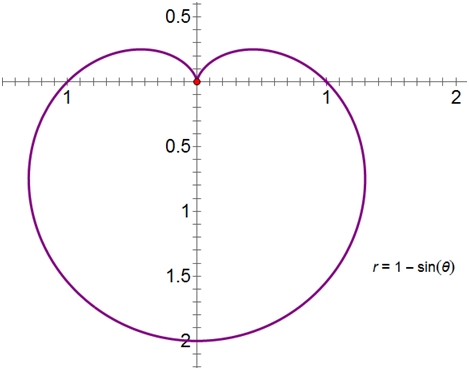
\includegraphics[scale=0.4]{r=1-sintheta.png}
			\caption{笛卡尔心形线~~~~~~}
		\end{figure}

	\end{center}


\end{frame}


\begin{frame}
	如果复数
\[
\alpha= |\alpha|(\cos \varphi+\i \operatorname{sin} \varphi), \quad
\beta=|\beta|(\cos \psi+\i \operatorname{sin} \psi),
\]
那么它们的乘积
	\[
	\begin{aligned}
		\alpha \beta &=|\alpha||\beta|(\cos \varphi+\i \operatorname{sin} \varphi)(\cos \psi+ i \operatorname{sin} \psi) \\
		&=|\alpha||\beta|(\cos \varphi \cos \psi-\sin \varphi \sin \psi)+(\sin \varphi \cos \psi+\cos \varphi \sin \psi) {\i}) \\
		&=|\alpha||\beta|(\cos (\varphi+\psi)+ \i \operatorname{sin}(\varphi+\psi))
	\end{aligned}
	\]
	上式表示,两个\alert{复数相乘}时,
    \begin{itemize}
    \item 其\blue{模}为这两个复数的模相乘,
    \item 其\blue{辐角}相 加(因为三角函数以 2 $\pi$ 为周期,故把相差 2 $\pi$ 的整数倍的角认为是相 同的).
    \end{itemize}
\end{frame}

\begin{frame}{欧拉公式}
	令模为 1的复数
	\[
	{{\e}^{{\i} \varphi}=\cos \varphi+{\i} \sin \varphi},
	\]
	上式称为\alert{欧拉公式}.

	因而位于以坐标原点 O 为中心的单位圆上,  其辐角为 $\varphi$. 于是
	\[
	{{\e}^{\i \varphi} {\e}^{{\i} \psi}={\e}^{{\i}(\varphi+\psi)}}.
	\]


	当$\varphi$为$\pi$时, $$\alert{\e^{\i\pi }=-1}.$$
	将数学内4个极重要的数$\e, \i, \, \pi,\,  -1 $连起来.
\end{frame}



\begin{frame}{方程$x^{\, n}-1=0$的解}
	给定一个正整数 $n$,考虑下面 $n$ 个复数
	\[
	\blue{x_k := {\e}^{\frac{2 k \pi }{n}{\i}}=\cos \frac{2 k \pi}{n}+\i\operatorname{sin} \frac{2 k \pi}{n}},
	\]
	其中 $k=0,1,2, \cdots, n-1.$

     这 $n$ 个复数就是以原点 $O$ 为中心的单 位圆的内接正 $n$ 边形的 $n$ 个顶点.
	由欧拉公式可知,
	\[
	\left({\e}^{\frac{2 {k\pi }}{n}i}\right)^{n}=\left(\cos \frac{2 k \pi}{n}+\i \operatorname{sin} \frac{2 k \pi}{n}\right)^{n}=\cos 2 k \pi+{\i} \sin 2 k \pi=1.
	\]
	因此, 这$n$ 个复数
%    $\blue{{\e}^{\frac{2 k \pi}{n} \i}=\cos \frac{2 k \pi}{n} + \i\,  \sin \frac{2 k \pi}{n}}$
    恰为 $n$ 次代数方程 $$\alert{x^{\,n}-1=0}$$ 在复数系 $\mathbb{C}$ 内的 $n$ 个根,称为 \blue{$n$ 次单位根}.

%    它们是很有用的工
%	具, 在许多问题中都会用到.
\end{frame}

%
%\begin{frame}
%\begin{equation}
%	\frac{d v^{2}}{d t}=2 v \frac{d v}{d t}=2 v \dot{v}
%\end{equation}
%
%\begin{equation}
%	D^{+}\left|\eta_{i}(t)\right| \leq e^{t}\left\{-h_{i}\left|\eta_{i}(t)\right|+\left|\varepsilon_{i}(t)\right|\right\}
%\end{equation}
%
%\begin{equation}
%	e^{\int_{x}^{y} \frac{\theta s}{(1-a) \lambda \mu^{2}} d s}
%\end{equation}
%
%\end{frame}




\begin{frame}
    \tableofcontents
\end{frame}
\AtBeginSection[]
{
    \begin{frame}
        \frametitle{Outline}
        \tableofcontents[currentsection]
    \end{frame}
}
\section{二项式系数}



\begin{frame}
    %

    二项式定理中的系数 都是组合数,组合数和二项式定理有密切的关系.

    本章我们就详细讨论这种关系.


    回忆:  表达式$\binom{n}{k}$表示 $n$元集合的$k$-组合数.




    %由于它们出现在二项式定理中,因此也叫做二项式系数.

    对于非负整数$n$和$k$, 我们已经证明了\vspace{8pt}
    $$
    \binom{n}{k}=\left\{\begin{array}{cc}
        \frac{n!}{k!(n-k)!} &1 \le {k} \le {n}
        \\[6pt]
        {0} & {k}>n
        %        \\[6pt]
        %        {0} & {k} < 0
    \end{array}\right.$$

    由此 不难得到


    \begin{itemize}

        \item 对称性:  $\binom{n}{k}=\binom{n}{n-k}$

        \item 恒等式: $\binom{n}{0}+\binom{n}{1}+\cdots+\binom{n}{n}=2^{n}$


    \end{itemize}


    它还具有许多很奇妙的性质,关于它也有着许多恒等式.
    %当$k>n$时,  ${n \choose k}=0.$

    %当$0 \le k \le n$时,
    %\[\binom{n}{k}=\frac{n!}{k!(n-k)!}\]

    %特别地,
    %$${n \choose 0}={n \choose n}=1$$
\end{frame}


\begin{frame}
    %    {Pascal公式}



    Pascal公式给出了二项式系数的\blue{递推关系}.
    \begin{thm}[Pascal公式]

        对于满足$1\leq k\leq n-1$的所有整数$k$和$n$,
        \[
        \binom{n}{k}=\binom{n-1}{k}+\binom{n-1}{k-1}.
        \]
    \end{thm}
    %
    %\blue{边值条件}
    %${n \choose 0}={n \choose n}=1$
    %


    利用\blue{边值条件}
    ${n \choose 0}={n \choose n}=1$  和 Pascal公式 可以得到下面的表格:
    \begin{table}[]
        \begin{tabular}{c|cccccc}
            $n\backslash k$ & 0 & 1 & 2  & 3  & 4 & 5 \\ \hline
            0 & 1 &   &    &    &   &   \\
            1 & 1 & 1 &    &    &   &   \\
            2 & 1 & 2 & 1  &    &   &   \\
            3 & 1 & 3 & 3  & 1  &   &   \\
            4 & 1 & 4 & 6  & 4  & 1 &   \\
            5 & 1 & 5 & 10 & 10 & 5 & 1 \\
        \end{tabular}
        \caption{Pascal三角}
    \end{table}

    \vspace{-10pt}


    \pause
    证明:直接将$\binom{n}{k}=\frac{n!}{k!\cdot(n-k)!}$代入上式验证等式成立.
\end{frame}



\begin{frame}
%    {Pascal三角  (杨辉三角 或 贾宪三角)}
    \begin{center}
        \begin{minipage}{0.55\linewidth}
            17世纪, 法国数学家Pascal做出了下面的三角形.
            %        ,西方通常叫做Pascal三角.
            \begin{table}[]
                \begin{center}
                    1

                    1 \quad 1

                    1\quad	\quad2\quad	\quad1

                    1\quad	\quad  3\quad\quad3\quad\quad	1

                    1\quad	\quad 4 \quad\quad	6\quad\quad	4\quad \quad	1

                    1\quad\quad	5\quad\quad	10\quad\quad	10\quad\quad	5\quad\quad	1

                    1\quad\quad	6\quad\quad	15\quad\quad	20\quad\quad	15\quad\quad	6\quad\quad	1

                \end{center}
                \caption{Pascal三角}
                %    \caption{杨辉三角 或 贾宪三角}
            \end{table}
        \end{minipage}
        \hspace*{25pt}
        \begin{minipage}{0.35\linewidth}
            \begin{figure}
                \centering
                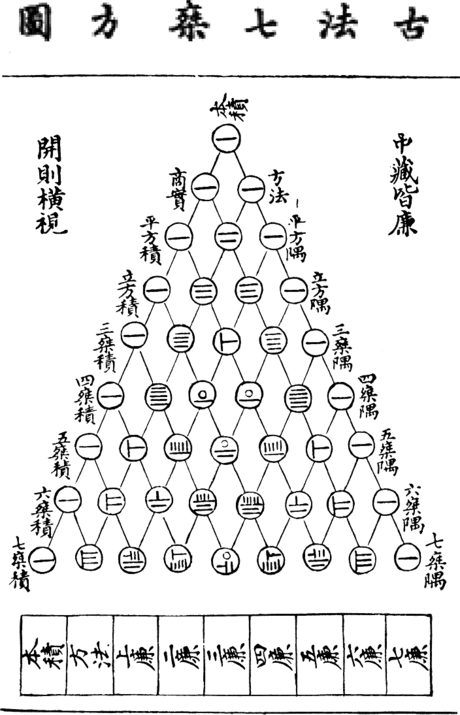
\includegraphics[scale=0.21]{yanghui.png}
                \caption{朱世杰《四元玉鉴》中的“古法七乘方图''}
            \end{figure}
        \end{minipage}
    \end{center}






    13世纪中国南宋数学家杨辉在《详解九章算术》里解释右边这种形式的数表,并说明此表引自11世纪贾宪的《释锁算术》.

    %贾宪还对贾宪三角表(古代称数字表为“立成”)的构造进行描述.
    %贾宪的三角表图和文字描写,仍保存在大英博物馆所藏《永乐大典》卷一万六千三百四十四.


    %在我国称这个三角形为杨辉三角形, 1250年由杨辉提出.
\end{frame}



%\begin{frame}{$\binom{n}{k}=\binom{n-1}{k}+\binom{n-1}{k-1}$的组合证明}
%
%
%\begin{minipage}{0.48\linewidth}
%	\begin{itemize}
    %	\item 令$S$是$n$元集合,
    %    考虑它的$k$-组合
    %
    %    \item 任取$x \in S$,将$S$的$k$-组合按$x$分成两大类:
    %        \begin{center}
        %        $A$ \, =\, \{不含元$x$的$k$-组合\} \\
        %        $B$ \, =\, \{包含元$x$的$k$-组合\}
        %        \end{center}
    %    \item  按加法原理,$\binom{n}{k}=|A|+|B|$
    %
    %	\item $A$的$k$-组合恰好是集合$S-\{x\}$的$k$-组合,故$$|A|=\binom{n-1}{k}$$
    %
    %
    %\item  $B$的$k$-组合是通过将$x$添加到集合$S-\{x\}$的($k-1$)-组合得到的,故$$|B|=\binom{n-1}{k-1}.$$
    %	\end{itemize}
%\end{minipage}
%\begin{minipage}{0.5\linewidth}
%\begin{flushleft}
%\quad 例如:
%
%\begin{itemize}
%\item $S=\{x,a,b,c,d\}$,
%
%$n=5$,$k=3$,$\binom{n}{k}=10$
%
%
%\item $A$的3-组合:
%
%\begin{center}
%$\{a,b,c\}$, $\{a,b,d\}$,
%
%$\{a,c,d\}$, $\{b,c,d\}$,
%\end{center}
%
%对应集合$\{a,b,c,d\}$的3-组合
%
%
%\item  $B$的3-组合:
%
%\begin{center}
%$\{x,a,b\}$, $\{x,a,c\}$, $\{x,a,d\},$
%
%$\{x,b,c\}$, $\{x,b,d\}$, $\{x,c,d\}$,
%\end{center}
%
%
%去掉$x$后,得
%
%\begin{center}
%$\{a,b\}$, $\{a,c\}$, $\{a,d\}$,
%
%$\{b,c\}$, $\{b,d\}$, $\{c,d\}$,
%\end{center}
%
%恰好是集合$\{a,b,c,d\}$的2-组合.
%\end{itemize}
%
%\end{flushleft}
%\end{minipage}
%
%
%\end{frame}

\begin{frame}{$\binom{n}{k}=\binom{n-1}{k}+\binom{n-1}{k-1}$的组合证明 --- 集合的组合}


    \begin{minipage}{0.49\linewidth}
        \begin{itemize}
            \item 令$S=\{1,2,\cdots,n\}$,\\
            考虑它的$k$-组合

            \item 将$S$的$k$-组合分成两类:
            \begin{center}
                $A$ \, =\, \{不含元$n$的$k$-组合\} \\
                $B$ \, =\, \{包含元$n$的$k$-组合\}
            \end{center}
            \item  按加法原理,$\binom{n}{k}=|A|+|B|$.

            \item $A$的$k$-组合恰好是集合 $\{1,2,\cdots,n-1\}$的$k$-组合,故$|A|=\binom{n-1}{k}$


            \item  $B$的$k$-组合已包含$n$,只需从集合$\{1,2,\cdots,n-1\}$中再选出 $k-1$个元素即可,故$|B|=\binom{n-1}{k-1}.$
        \end{itemize}
    \end{minipage}
    \begin{minipage}{0.49\linewidth}
        \begin{flushleft}
            \quad 例如:

            \begin{itemize}
                \item  $n=5$,$k=3$,$\binom{n}{k}=10$

                $S=\{1,2,3,4,5\}$,




                \item

                \small{$A$的3-组合:

                \begin{center}
                    $\{1,2,3\}$, $\{1,2,4\}$,

                    $\{1,3,4\}$, $\{2,3,4\}$,
                \end{center}

                对应集合$\{1,2,3,4\}$的3-组合.}


                \item  \small{$B$的3-组合:

                \begin{center}
                    $\{1,2,5\}$, $\{1,3,5\}$, $\{1,4,5\},$

                    $\{2,3,5\}$, $\{2,4,5\}$, $\{3,4,5\}$,
                \end{center}


                去掉$n=5$后,得

                \begin{center}
                    $\{1,2\}$, $\{1,3\}$, $\{1,4\}$,

                    $\{2,3\}$, $\{2,4\}$, $\{3,4\}$,
                \end{center}

                恰好是集合$\{1,2,3,4\}$的2-组合.}
            \end{itemize}

        \end{flushleft}
    \end{minipage}


\end{frame}


\begin{frame}{$\binom{n}{k}=\binom{n-1}{k}+\binom{n-1}{k-1}$的另一种组合解释}

    \begin{itemize}

        \item 令$n$是非负整数,且$1\leq k\leq n-1$.

        \item  $p(n,k):$表示从点$(0,0)$到点$(k,n-k)$的路径的条数,其中

        每条路径包含$n$步,每一步只有两种选择:
        \begin{center}
            水平向右$(1,0) \rightarrow$\quad \quad  水平向上$(0,1) \uparrow$
        \end{center}


        \item 从点$(0,0)$到点$(k,n-k)$的路径,有两种选择

        $i)$从点(0,0)到点$(k,n-k-1)$,再水平向上移至$(k,n-k)$;

        $ii) $从点$(0,0)$到点$(k-1,n-k)$,再水平向右移至$(k,n-k)$;

        \item 由加法原理:$p(n,k)=p(n-1,k)+p(n-1,k-1)$.

        %        \item 即$p(n,k)$与$\binom{n}{k}$有相同的递推式和相同的初值,从而$p(n,k)=\binom{n}{k}$

    \end{itemize}
    \begin{figure}
        \centering
        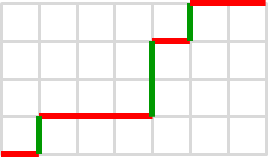
\includegraphics[scale=0.3]{path.png}
        \caption{格路}
    \end{figure}
\end{frame}




\begin{frame}
\begin{minipage}{0.65\linewidth}
    \begin{table}[]
        \begin{tabular}{c|cccccccc}
            $n\backslash k$ & 0 & 1 & 2  & 3  & 4 & 5 & 6 & 7 \\ \hline
            0 & 1 &   &    &    &   &   & 	& \\
            1 & 1 & 1 &    &    &   &   & 	& \\
            2 & 1 & 2 &\cellcolor{green}1  &    &   &   & 	& \\
            3 & 1 & 3 & \cellcolor{green}3  & 1  &   &   &	& \\
            4 & 1 & 4 & \cellcolor{green}6  & 4  & 1 &   &  & \\
            5 & 1 & 5 & \cellcolor{green}10 & 10 & 5 & 1 & & \\
            6 & 1 & 6 & \cellcolor{green}15 & 20 & 15 & 6 & 1&  \\
            7 & 1 & 7 & 21 & \cellcolor{red}35 & 35 & 21 & 7 & 1\\
        \end{tabular}
        %	    	\caption{Pascal三角}
    \end{table}
\end{minipage}
\begin{minipage}{0.3\linewidth}
    \begin{figure}
        \centering
        
\includegraphics[scale=0.3]{HockeyStick.png}
    \end{figure}
\end{minipage}

一般地,可以得到
\begin{block}{朱世杰恒等式}
    设$n,k$是两个正整数.
    若$n>k$, 则
    $$\sum_{i=k}^{n}\binom{i}{k}=\binom{n+1}{k+1}.$$
\end{block}

一些英文教材上常称这个恒等式为 Hockey-stick identity.

% 提示: 关于$n$做数学归纳法.
\end{frame}

%\begin{frame}
%	\begin{table}[]
%		\begin{tabular}{c|cccccccc}
    %			$n\backslash k$ & 0 & 1 & 2  & 3  & 4 & 5 & 6 & 7 \\ \hline
    %			0 & 1 &   &    &    &   &   & 	& \\
    %			1 & 1 & 1 &    &    &   &   & 	& \\
    %			2 & 1 & 2 &\cellcolor{green}1  &    &   &   & 	& \\
    %			3 & 1 & 3 & \cellcolor{green}3  & 1  &   &   &	& \\
    %			4 & 1 & 4 & \cellcolor{green}6  & 4  & 1 &   &  & \\
    %			5 & 1 & 5 & \cellcolor{green}10 & 10 & 5 & 1 & & \\
    %			6 & 1 & 6 & \cellcolor{green}15 & 20 & 15 & 6 & 1&  \\
    %			7 & 1 & 7 & 21 & \cellcolor{red}35 & 35 & 21 & 7 & 1\\
    %		\end{tabular}
%		\caption{Pascal三角}
%	\end{table}
%\end{frame}



\begin{frame}
\begin{ex}
    利用\[m^{2}=2\binom{m}{2}+\binom{m}{1} \]	计算$1^{2}+2^{2}+\cdots+n^{2}$的值.
\end{ex}
\pause
\[
\begin{aligned}
    1^{2}+2^{2}+\cdots+n^{2}
    &=\sum_{m=1}^{n}m^{2}
    =2\sum_{m=1}^{n}\binom{m}{2}+\sum_{m=1}^{n}\binom{m}{1}\\
    &=2\binom{n+1}{3}+\binom{n+1}{2}\\
    &=\frac{1}{6}n\, (n+1)\, (2n+1).
\end{aligned}
\]
\end{frame}


\begin{frame}
\begin{ex}
    求整数$a,b,c$使得\[m^{3}=a\binom{m}{3}+b\binom{m}{2}+c\binom{m}{1}\tag{*}\]并计算$1^{3}+2^{3}+\cdots+n^{3}$的值.
\end{ex}
\pause
将$m=1,2,3$分别代入(*)式得
\begin{align*}
    1 = &\,  c \\
    8 = &\,  b+2 c \\
    27 = &\,   a+3 b+3 c
\end{align*}

解方程组得$a=6,b=6,c=1$.

\end{frame}

\begin{frame}
\begin{block}{例}
    求整数$a,b,c$使得\[m^{3}=a\binom{m}{3}+b\binom{m}{2}+c\binom{m}{1}\tag{*}\]并计算$1^{3}+2^{3}+\cdots+n^{3}$的值.
\end{block}
\[m^{3}=6\binom{m}{3}+6\binom{m}{2}+\binom{m}{1}\]
因此,
\begin{align*}
    1^{3}+2^{3}+\cdots+n^{3} &=\sum_{m=1}^{n} m^{3}
    =6 \sum_{m=1}^{n}\binom{m}{3} +6 \sum_{m=1}^{n} \binom{m}{2}+\sum_{m=1}^{n}\binom{m}{1}\\
    &=6\binom{n+1}{4}+6\binom{n+1}{3}+\binom{n+1}{2} \\
    &=\frac{1}{4} n^{2}(n+1)^{2}
\end{align*}
\end{frame}

\begin{frame}
清代数学家李善兰(1811-1882)在 《垛积比类》一书中对垛积进行了系统 的研究.所谓垛积数就是二项式系数, 因用于计算按照一定图形堆垛的物品 数量而得其名.在该书的第二卷, 李善兰讨论了如下的求和问题:
$$
1^p+2^p+\cdots+n^p,
$$
其中 $p$ 为正整数.为此他把 $m^p$ 分解成垛积数 $\binom{ m+p-k}{p}$ 的线性组合
$$
m^p=\sum_{k=1}^p A(p, k) \binom{ m+p-k}{p}, \quad m=1,2, \ldots, n,
$$
其中 $A(p, k)$ 为与 $m$ 无关的系数, 称为李善兰系数.

闻名中外的 “李善兰恒等 式” 就是从上述分解过程中归纳得到的:
$$
\sum_{k=0}^m \binom{m}{k}^2
\binom{n+2 m-k}{2 m}
=\binom{m+n
}{n}^2 .
$$

Andrews 称上述恒等式为中国恒等式(Chinese Identity).

华罗庚给 出了这个恒等式的数学归纳法证明.
\end{frame}


\begin{frame}
\begin{block}{二十大报告}
要坚持教育优先发展、科技自立自强、人才引领驱动,
加快建设教育强国、科技强国、人才强国,
坚持为党育人、为国育才,
全面提高人才自主培养质量,
着力造就拔尖创新人才,
聚天下英才而用之.
\end{block}


\begin{block}{2013年5月4日习近平同各界优秀青年代表座谈时的讲话}
     青年人正处于学习的黄金时期, 应该把学习作为首要任务, 作为一种责任、一种精神追求、一种生活方式, 树立梦想从学习开始、事业靠本领成就的观念, 让勤奋学习成为青春远航的动力, 让增长本领成为青春搏击的能量.
\end{block}
\end{frame}
\end{document}